%\documentclass{article}
\documentclass[letterpaper]{article}
\usepackage{ijcai13}
\usepackage{times}
\usepackage{array}
\usepackage[utf8]{inputenc}
\usepackage[table]{xcolor}
\usepackage{amsmath}
\usepackage{amssymb}
\usepackage{graphicx}        % standard LaTeX graphics tool                            % when including figure files
\usepackage{multicol}        % used for the two-column index
\usepackage{multirow}
\usepackage{lscape}
\usepackage{float}
\usepackage{url}
\usepackage{caption,subfig}

%\usepackage{epstopdf} 

\makeatletter
\def\blfootnote{\xdef\@thefnmark{}\@footnotetext}
\makeatother

\setlength{\pdfpagewidth}{8.5in}
\setlength{\pdfpageheight}{11in}
\pdfinfo{
/Title (Pareto-Based Multiobjective AI Planning)
/Author (Mostepha-Redouane Khouadjia, Marc Schoenauer, Vincent Vidal, Johann Dr\'eo, Pierre Sav\'eant)
}

% Please leave SVN version number $Revision$
% et ne pas oublier svn propset svn:keywords "Revision"  thisFile.tex:
\title{Pareto-Based Multiobjective AI Planning}

\author{\hspace{5mm}Mostepha Khouadjia ~~ Marc Schoenauer\\ TAO Project, INRIA Saclay\\ LRI Paris-Sud University, Orsay, France\\ first.last@inria.fr
\And Vincent Vidal \\ ONERA\\ Toulouse, France \\ Vincent.Vidal@onera.fr
\And Johann Dr\'eo ~~ Pierre Sav\'eant\\ Thales Research \& Technology \\ Palaiseau, France\\ first.last@thalesgroup.com
}


% macros from ijcai2013 paper
\def\dae{{\em Divide-and-Evolve}}
\def\DAE{{\sc DaE}}
\def\DAEX{{\sc DaE$_{\text{X}}$}}
%\def\DAEYAHSP{{\sc DaE$_{\text{YAHSP}}$}}
\newcommand{\DAEYAHSP}{{\sc DaE$_{\text{YAHSP}}$}}
\def\PARADISEO{{\sc ParadisEO-MOEO}}
\def\YAHSP{{\sc YAHSP}}
\def\CPT{{\sc CPT}}
\def\modae{{\em Multiobjective Divide-and-Evolve}}
\def\MODAE{{\sc MO-DaE}}
\newcommand{\MODAEYAHSP}{{\sc MO-DaE$_{\text{YAHSP}}$}}
\newcommand{\MODAEX}{{\sc MO-DaE$_{\text{X}}$}}
\newcommand{\MOLPG}{{\sc MO-LPG}}
\def\ZENO{{\sc Zeno}}
\def\MULTIZENO{{\sc MultiZeno}}
\def\PARAMILS{{\sc ParamILS}}
\def\IBEAH{{\sc IBEA$_{\text{H}}$}}

\def\WMAKESPAN{{W-makespan}}
\def\WCOST{{W-cost}}

\newcommand{\ZENOTRAVEL}{{\sc ZenoTravel}}
\newcommand{\OPENSTACKS}{{\sc Openstacks}}
\newcommand{\ELEVATORS}{{\sc Elevators}}
\newcommand{\CREWPLANNING}{{\sc CrewPlanning}}
\newcommand{\FLOORTILE}{{\sc Floortile}}
\newcommand{\PARCPRINTER}{{\sc ParcPrinter}}

\newcommand{\mycomments}[1]{\textcolor{red}{#1}}
% \newcommand{\mycomments}[1]{~}

\begin{document}

\maketitle

\begin{abstract}
Real-world problems generally involve several antagonistic objectives, like quality and cost for design problems, or makespan and cost for planning problems. The only approaches to multiobjective AI Planning rely on metrics, that can incorporate several objectives in some linear combinations, and metric sensitive planners, that are able to give different plans for different metrics, and hence to eventually approximate the Pareto front of the multiobjective problem, i.e. the set of optimal trade-offs between the antagonistic objectives. Divide-and-Evolve (\DAE) is an evolutionary planner that embeds a classical planner and feeds it with a sequence of subproblems of the problem at hand. Like all Evolutionary Algorithms, \DAE\ can be turned into a Pareto-based multiobjective solver, even though using an embedded planner that is not metric sensitive. The Pareto-based multiobjective planner \MODAE\ thus avoids the drawbacks of the aggregation method. Furthermore, using YAHSP as the embedded planner, it 
outperforms 
in many cases the metric-based approach using LPG metric sensitive planner, as witnessed by experimental results on original multiobjective benchmarks built upon IPC-2011 domains.\blfootnote{This work was partially funded by the DESCARWIN ANR project (ANR-09-COSI-002).}
\end{abstract}

\section{Introduction}

Multiobjective problems are ubiquitous in the real world, where most situations often involve at least two antagonistic objectives, such as maximizing some quality criterion (or even criteria) while minimizing some costs --  and quality increase cannot be obtained without corresponding cost increase. This is true in AI planning too, as witnessed by looking at the most popular test problems that have been used in IPC competitions. Many domains have been defined in both categories of actions with cost and temporal planning: the more general problem is to minimize both the makespan (where high quality solutions correspond to small makespan values) and the cost of a given plan, while these two objectives are in general antagonistic\footnote{Though some costs might be proportional to durations in some domains.}. 

Given two solutions $A$ and $B$ of such multiobjective problems, $A$ is obviously to be preferred to $B$ in the case when the objective values for $A$ are all better than the objective values of $B$: in such case, $A$ is said to Pareto-dominate $B$. However, Pareto-dominance is not a total order, and most solutions are not comparable for this relationship. The set of interest when facing a multiobjective problem is the so-called {\em Pareto set} of all solutions of the search space that are not dominated by any other solution: such non-dominated solutions are the best possible trade-offs between the antagonistic objectives, in that there is no way to improve on one objective without degrading at least another one. Figure \ref{fig:hypervolume} depicts a simple case of a two objectives AI Planning problem, and presents both the {\em design space}, space of solutions plans, and its projection on the {\em objective space}, here the $(\mbox{makespan} \times \mbox{cost})$ space (both to be minimized). The {\em 
Pareto front} (circles on the right figure) is the image of the Pareto set in the objective space.

\begin{figure}[h!]
\centerline{ 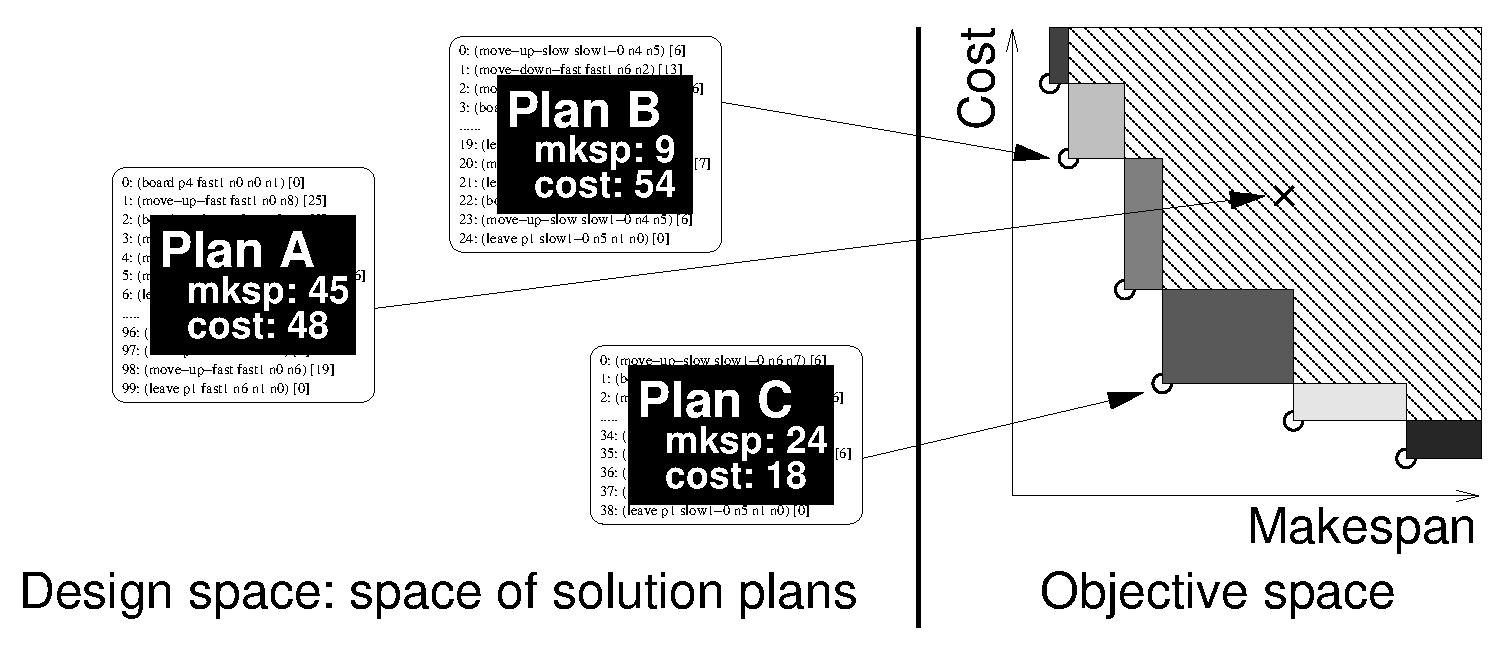
\includegraphics[width=.99\columnwidth]{figures/hypervolumeContributionDAE-V2}}
\caption{Design and objective spaces for a two-objectives planning problem. The hatched+grey area contains all images of possible solutions plans; this area defines the {\em hypervolume} of the set of circles, and the {\em hypervolume contribution} of each point is the grey area of the corresponding small rectangle (see Section \ref{sec:pareto}). Circles are Pareto-optimal (non-dominated) solutions, aka the {\em Pareto front} of the problem at hand.}
\label{fig:hypervolume}
\end{figure}


Sometimes, the user/decision maker might have a very precise idea of the relative losses induced by the degradation of one of the objectives with respect to the improvement of another. It is then possible to turn the multiobjective optimization problem into a single-objective optimization problem, e.g., by optimizing some weighted sum (or any other monotonous function) of the objectives, in the so-called {\em aggregation method}. Any optimizer can then be used to solve the aggregated problem. However, this approach requires some a priori knowledge of the trade-off between the objectives, and/or numerous runs of the optimizer on different aggregations of the objectives. Furthermore, linear aggregation (the weighted sum case) is not able to identify the complete Pareto front in case it is not convex. 

To address this multidimensional issue, Pareto-based algorithms have been designed in order to directly identify the complete Pareto front, by computing a set of approximate non-dominated solutions.
This one can then be offered to the decision maker so that she/he can make an informed decision when choosing a solution. 
Efficient Pareto-based multiobjective algorithms have been designed using ideas from Evolutionary Algorithms, that can easily be turned into Multiobjective Evolutionary Algorithms (MOEAs) by modifying their selection process to account for Pareto dominance \cite{Deb-book}.

In the domain of AI planning, most works only address single-objective problems, and the very few recent approaches rely on {\em metric sensitive} planners to optimize metrics built as weighted sums of the objectives (more in Section \ref{sec:multi-planning}). 
This paper introduces \MODAE, the first (to the best of our knowledge) truly Pareto-based Multiobjective AI Planning System. \MODAE\ is a multi-objectivization of \DAE, a domain-independent satisficing planner that has been originally designed for single-objective planning \cite{evoCOP2006,Bibai2010}, and won the IPC-2011 temporal deterministic satisficing track at ICAPS 2011. \DAE\ uses an Evolutionary Algorithm (EA) to evolve sequences of partial states for the problem at hand, calling an embedded planner to solve in turn each subproblem of the sequence. If the embedded planner is able to compute metrics along any plan it builds, then \MODAE\ will take care of the global search for the Pareto front, without the need for the embedded planner to be metric sensitive. After a brief survey of Multiobjective Evolutionary Algorithms (MOEAs, Section \ref{sec:pareto}), Section \ref{sec:pareto-multi-planning} details \DAE\ and \MODAE.

Although there exist many single-objective planning benchmarks, thanks to the IPC competitions, none has been proposed yet for multiobjective planning. Both a specific tunable artificial benchmark, and a general method to turn some well-known IPC benchmarks into multiobjective domains are presented in Section \ref{sec:benchmarks}. In Section \ref{sec:experiments}, \MODAEYAHSP, the instantiation of \MODAEX\ with YAHSP \cite{Vidal2004} as the embedded planner, is validated on these instances, and compared to the metric-based approach using the metric sensitive planner LPG \cite{gerevini2008}, following \citeauthor{LPG-PlanSIG2012} [\citeyear{LPG-PlanSIG2012}]. Finally, Section \ref{sec:conclusion} discusses these results and sketches the directions for further research.

\section{Multiobjective AI Planning}
\label{sec:multi-planning}

Temporal planning and numerical state variables have been formalized in PDDL2.1 \cite{PDDL2}, as well as metric functions that allow to optimize an aggregation of some criteria based on time and numerical variables. This language has been extended  in PDDL3 \cite{gerevini2006preferences} in order to express preferences and soft constraints, which de facto increase the expressivity and complexity of the metric function to be optimized. However, even though optimizing such functions is a standard way to tackle multiobjective optimization problems, its extension to Pareto-based multiobjective optimization is not straightforward and nothing had been proposed in AI Planning for that purpose until very recently. Indeed, all the literature about multi-criteria/objective planning, such as the works on the planners GRT \cite{Refanidis03}, SAPA \cite{Do2003sapa} or LPG \cite{gerevini2008}, are concerned with optimizing an aggregation of the objectives.

The concept of metric sensitive planners has been recently defined in \citeauthor{LPG-STAIRS2012} [\citeyear{LPG-STAIRS2012}], in order to identify planners able to give diverse solutions when faced with -- possibly small -- variations of the metric function. With such a planner, the Pareto front can be approximated by adequately weighting an aggregation of the objectives and running the planner several times within some time limits. An example of such a metric function is $\alpha\times\mathtt{makespan}+(1-\alpha)\times\mathtt{cost}$, where alpha is sampled in $[0,1]$. The authors experimented several candidates and retained LPG which exhibited by far the best performance in terms of metric sensitivity and generated Pareto front quality \cite{LPG-PlanSIG2012}. 
For this reason, this approach, named here \MOLPG, will also be used as a baseline for the validation here (Section \ref{sec:experiments}). To overcome the metric insensitivity 
limitation of other planners, \citeauthor{LPG-STAIRS2012} [\citeyear{LPG-STAIRS2012}] suggest to add artificial bounds on numerical variables, which gave comparable results with the other 
planners in comparison with \MOLPG. However, this requires significantly more engineering, as defining the bounds requires an in-depth analysis of the planning problem, while defining objective weights is straightforward.


\section{Multiobjective Evolutionary Algorithms}
\label{sec:pareto}

Evolutionary Algorithms (EAs) \cite{EibenSmith2003} are heuristic stochastic search algorithms that crudely mimic natural evolution. A population of individuals (a set of potential solutions in the search space) evolves according to two main driving forces: reproduction through blind variations (random moves in the search space) and natural selection, aka ``survival of the fittest''. Blind variations depend on the search space, and are usually classified into crossover operators, that involve two or more parent individuals to create one offspring, and mutation operators, that modify a single parent to create one offspring. Selection is applied to choose which parents will reproduce, and also which from the parents plus offspring will survive to the next generation. It can be deterministic or stochastic, but has to be biased toward the fittest individuals. 

In the case of single-objective optimization of some objective function $\cal F$ (e.g., to be minimized), the fitness of an individual $x$ simply is the value ${\cal F}(x)$. In the case of multiobjective optimization, however, Pareto-dominance is not a total order, and hence cannot be used as sole selection criterion. Several Pareto-based Multiobjective Evolutionary Algorithms (MOEAs) have thus been proposed, that use some diversity measure as a secondary criterion when Pareto-dominance cannot distinguish between individuals. 

Several indicators have been proposed for comparing the results of different multiobjective optimization algorithms, i.e., that compare sets of solutions. The most popular is the {\em hypervolume indicator} (Figure \ref{fig:hypervolume}), because it is the only one that has been proved to-date to be consistent with the Pareto-dominance relation. But indicators can also be used to build a fitness function for some MOEAs: the fitness of an individual (compared to the other individuals in the population) is its contribution to the indicator of the population, i.e., the difference between the indicator of the whole population and that of the population without it. Such MOEAs are called {\em Indicator Based Evolutionary Algorithms} (IBEA) \cite{Zitzler2004} -- and \IBEAH, that will be used throughout this paper, is the one using the hypervolume indicator.


\section{Divide-and-Evolve}
\label{sec:DAE}

\subsection{Single-Objective Divide-and-Evolve}
This section introduces the main principles of the satisficing planner \DAE, referring to \cite{Bibai2010} for a comprehensive presentation.
Given a planning problem $P=\langle A, O, I, G\rangle$, where $A$ denotes the set of atoms, $O$ the set of actions, $I$ the initial state, and $G$ the goal state, \DAEX\ searches the space of sequences of partial states $(s_i)_{i\in [0,n+1]}$, with $s_0=I$ and $s_{n+1}=G$: \DAEX\ looks for the sequence such that the plan $\sigma$ obtained by compressing subplans $\sigma_i$ found by some embedded planner $X$ as solutions of $P_i=\langle A, O, \hat{s}_i, s_{i+1}\rangle_{i\in[0, n]}$ has the best possible quality (with $\hat{s_i}$ denoting the final state reached by applying $\sigma_{i-1}$ from $\hat{s}_{i-1}$). 
Each intermediate state $(s_i)_{i\in [1,n]}$ is first seen as a set of goals and then completed as a new initial state for the next step by simply applying the plan found to reach it.
In order to reduce the number of atoms used to describe these states, \DAE\ relies on the admissible heuristic function $h^1$ \cite{HaslumGeffner-AIPS-2000}: only the ones that are possibly true according to $h^1$ are considered.
Furthermore, mutually exclusive atoms, which can be computed at low cost, are also forbidden in intermediate states $s_i$. These two rules are strictly imposed during the random initialization phase, and progressively relaxed during the search phase.
The compression of subplans is required by temporal planning where actions can run concurrently: a simple concatenation would obviously not produce the minimal makespan.

Due to the weak structure of the search space (variable-length sequences of variable-length lists of atoms), Evolutionary Algorithms (EAs) have been chosen as the method of choice: EAs are metaheuristics that are flexible enough to explore such spaces, as long as they are provided with some stochastic {\em variation operators} (aka {\em move operators} in the heuristic search community) -- and of course some objective function to optimize. 

{\em Variation operators} in \DAE\ are (i) a crossover operator, a straightforward adaptation of the standard one-point crossover to variable-length sequences; and (ii) different mutation operators, that modify the sequence at hand either at 
the sequence level, or at the state level, randomly adding or removing one item (state or atom). 

The objective value is obtained by running the embedded planner on the successive subproblems. When the goal state is reached, a feasibility fitness is computed based on the compression of solution subplans, favoring quality; otherwise, an unfeasibility fitness is computed,  implementing a gradient towards satisfiability (see \cite{Bibai2010} for details).

\DAE\ can embed any existing planner, and has to-date been successful with both the optimal planner CPT \cite{vidal:aaai04} and the lookahead heuristic-based satisficing planner \YAHSP\ \cite{Vidal2004}. The latter has been demonstrated to outperform the former when used within \DAE\ \cite{bibai-EvoCOP2010}, so only \DAEYAHSP\ has been considered in this work.


\subsection{Multiobjective Divide-and-Evolve}
\label{sec:pareto-multi-planning}

Two modifications of \DAEYAHSP\ are needed to turn it into a MOEA: (i) use some multiobjective selection (Section \ref{sec:pareto}) in lieu of the single-objective tournament selection that is used in the single-objective context; (ii) use the embedded planner to compute the values of both objectives (e.g., makespan and cost). The former modification is straightforward, and several alternatives have been experimented within \cite{nous-emo2013}. The conclusion is that $IBEA_H$ \cite{Zitzler2004} (see Section \ref{sec:pareto}) performs best on instances \MULTIZENO\ (see Section \ref{sec:benchmarks}) -- and only this one will be mentioned in the following.

As explained above, the computation of the fitness is done by \YAHSP\ -- and \YAHSP, like all known planners to-date, is a single-objective planner. It is nevertheless possible, since PDDL 2.1, to specify other metrics that are to be computed throughout the execution of the final plan. For the metric sensitive planners, this metric is directly used to bias the search, while some other planners, like \YAHSP, simply compute it along the solution plan without interfering with the search. However, because \YAHSP\ is both a temporal planner and a cost planner, two strategies are possible for \YAHSP\ within \MODAE: it can be asked to optimize only the makespan (resp. the cost), and to simply compute the cost (resp. the makespan) when executing the solution plan. 

In \MODAEYAHSP, the choice between both strategies is governed by user-defined weights.
% , named respectively \WMAKESPAN\ and \WCOST. 
For each individual, the actual strategy is randomly chosen according to those weights, and applied to all subproblems of the individual. Another important feature of \YAHSP\ for the computation of the objectives of \MODAEYAHSP\ is its stochasticity: \YAHSP\ explores the plan space stochastically, and different runs on the same instance with different random seeds give different answers. This stochasticity, and the effect of the choice of \YAHSP\ strategy, % as well as \YAHSP\ 
can be observed on Figure \ref{fig:strategies}, that represent the different objective values of the same individual obtained within \MODAEYAHSP\ when \YAHSP\ uses either the makespan strategy, or the cost strategy, or strategies that are independently randomly chosen for each subproblem: the bias is clear when a unique strategy is chosen for the \MULTIZENO9 instance, and the corresponding part of the objective space is sampled, while the hybrid strategy spreads the values in-between these two clouds of points. Note that on some other instances (\OPENSTACKS, \FLOORTILE, see Section \ref{sec:benchmarks}), the three strategies are absolutely indistinguishable (not shown here).

Some preliminary experiments were also conducted in order to try to take advantage of the stochastic nature of \YAHSP\ evaluations, running \YAHSP\ several times for each individual and keeping the best plan. But surprisingly, even without considering the additional CPU cost, such approach proved detrimental on the quality of the Pareto approximation: such observation had also been made when trying to hybridize EAs with local search methods (iterated \YAHSP\ can indeed be viewed as some sort of local search) - the local search should not try to improve the solutions too early.

Final note regarding the evaluation: the strategy weights, like all parameters of \MODAEYAHSP, have been tuned using ParamILS (see Section \ref{sec:conditions}), and it turned out that the optimal values for \MODAEYAHSP\ have always been equal weights: something that was to be expected, as no objective should be preferred to the other. 

\section{Benchmark Domains and Instances}
\label{sec:benchmarks}
Two approaches were used to design multiobjective benchmark problems: first, using a highly simplified version of the well-known IPC domain \ZENOTRAVEL, a simple and easy to tune domain was built, and the exact Pareto front can be easily identified for all its instances. The other approach is based on modifying IPC-2011 problems.


\subsection{\MULTIZENO\ Instances}
\label{ZenoBenchmarks}
\begin{tiny}
\begin{figure}[tb]

\begin{tabular}{lr}
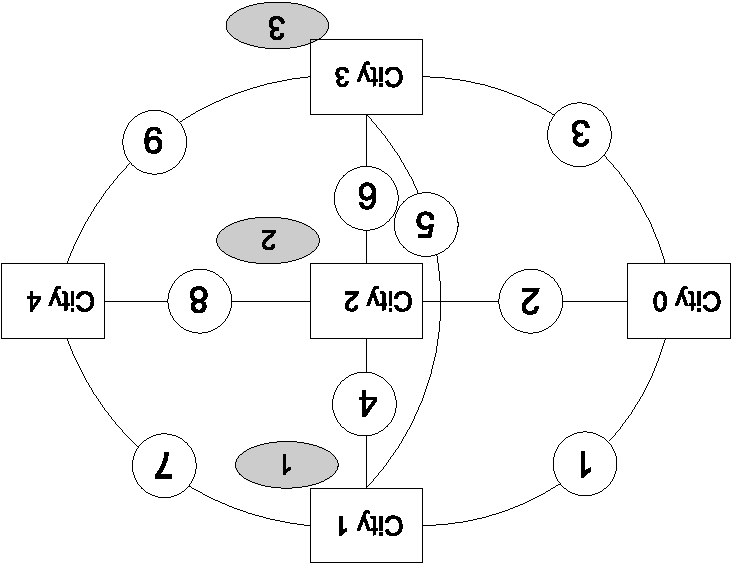
\includegraphics[height=0.47\columnwidth,angle=180]{figures/generiqueMiniMulti180}
%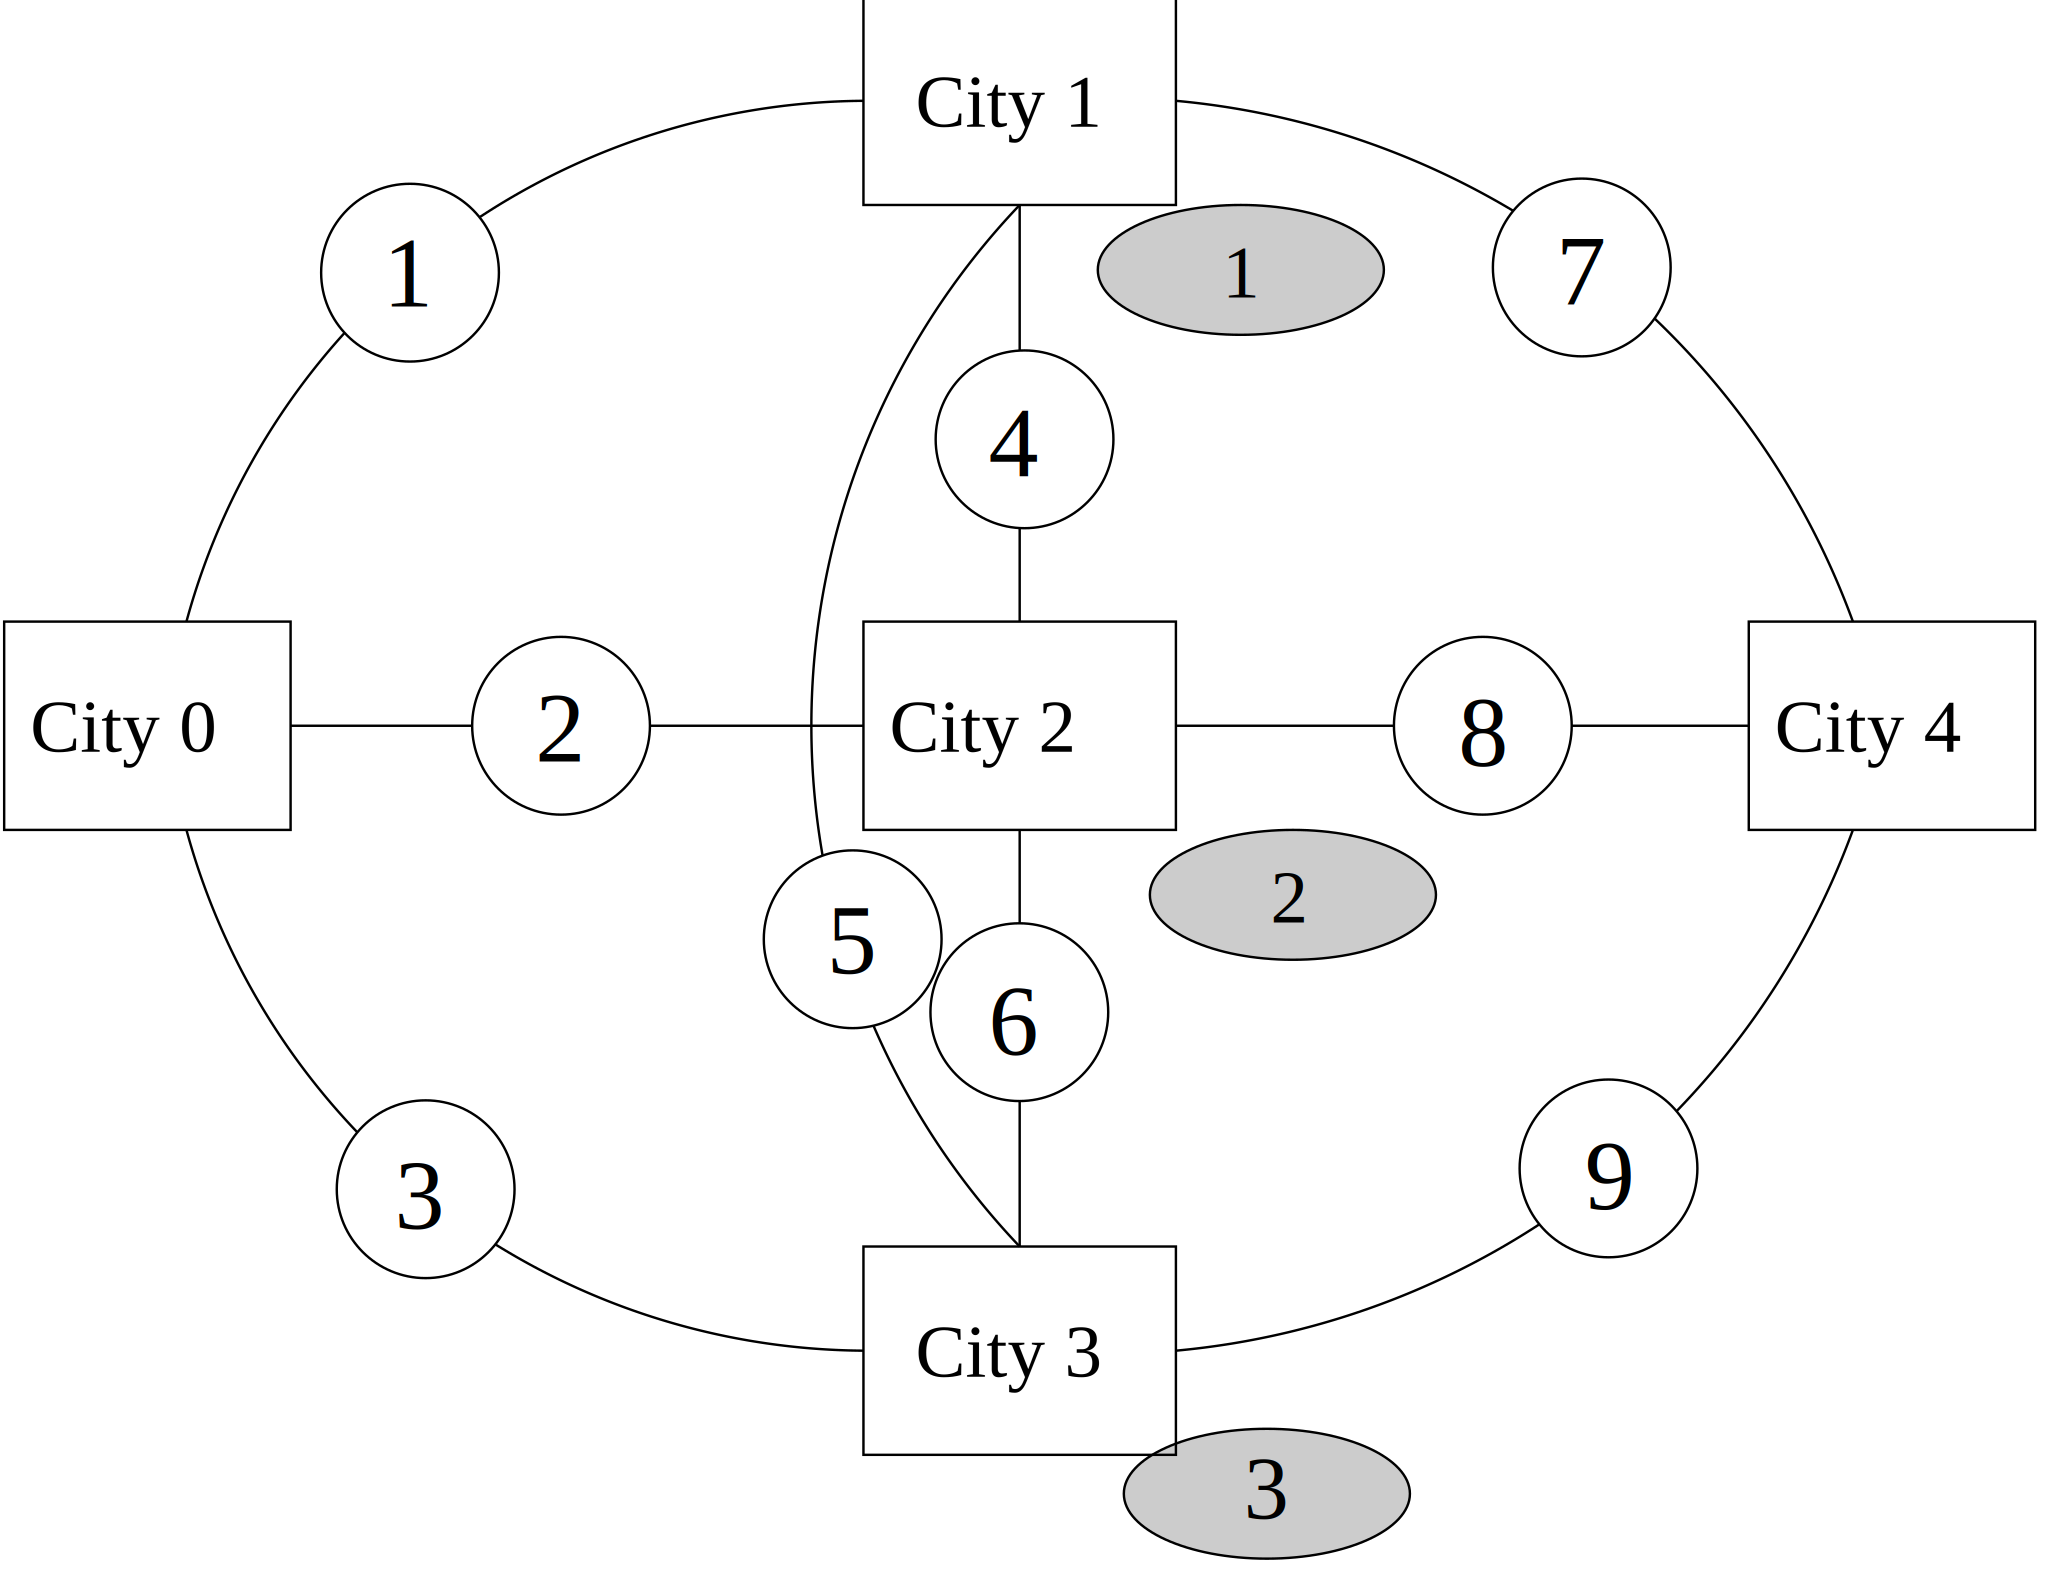
\includegraphics[width=0.6\columnwidth]{./generiqueMiniMulti}
%\framebox{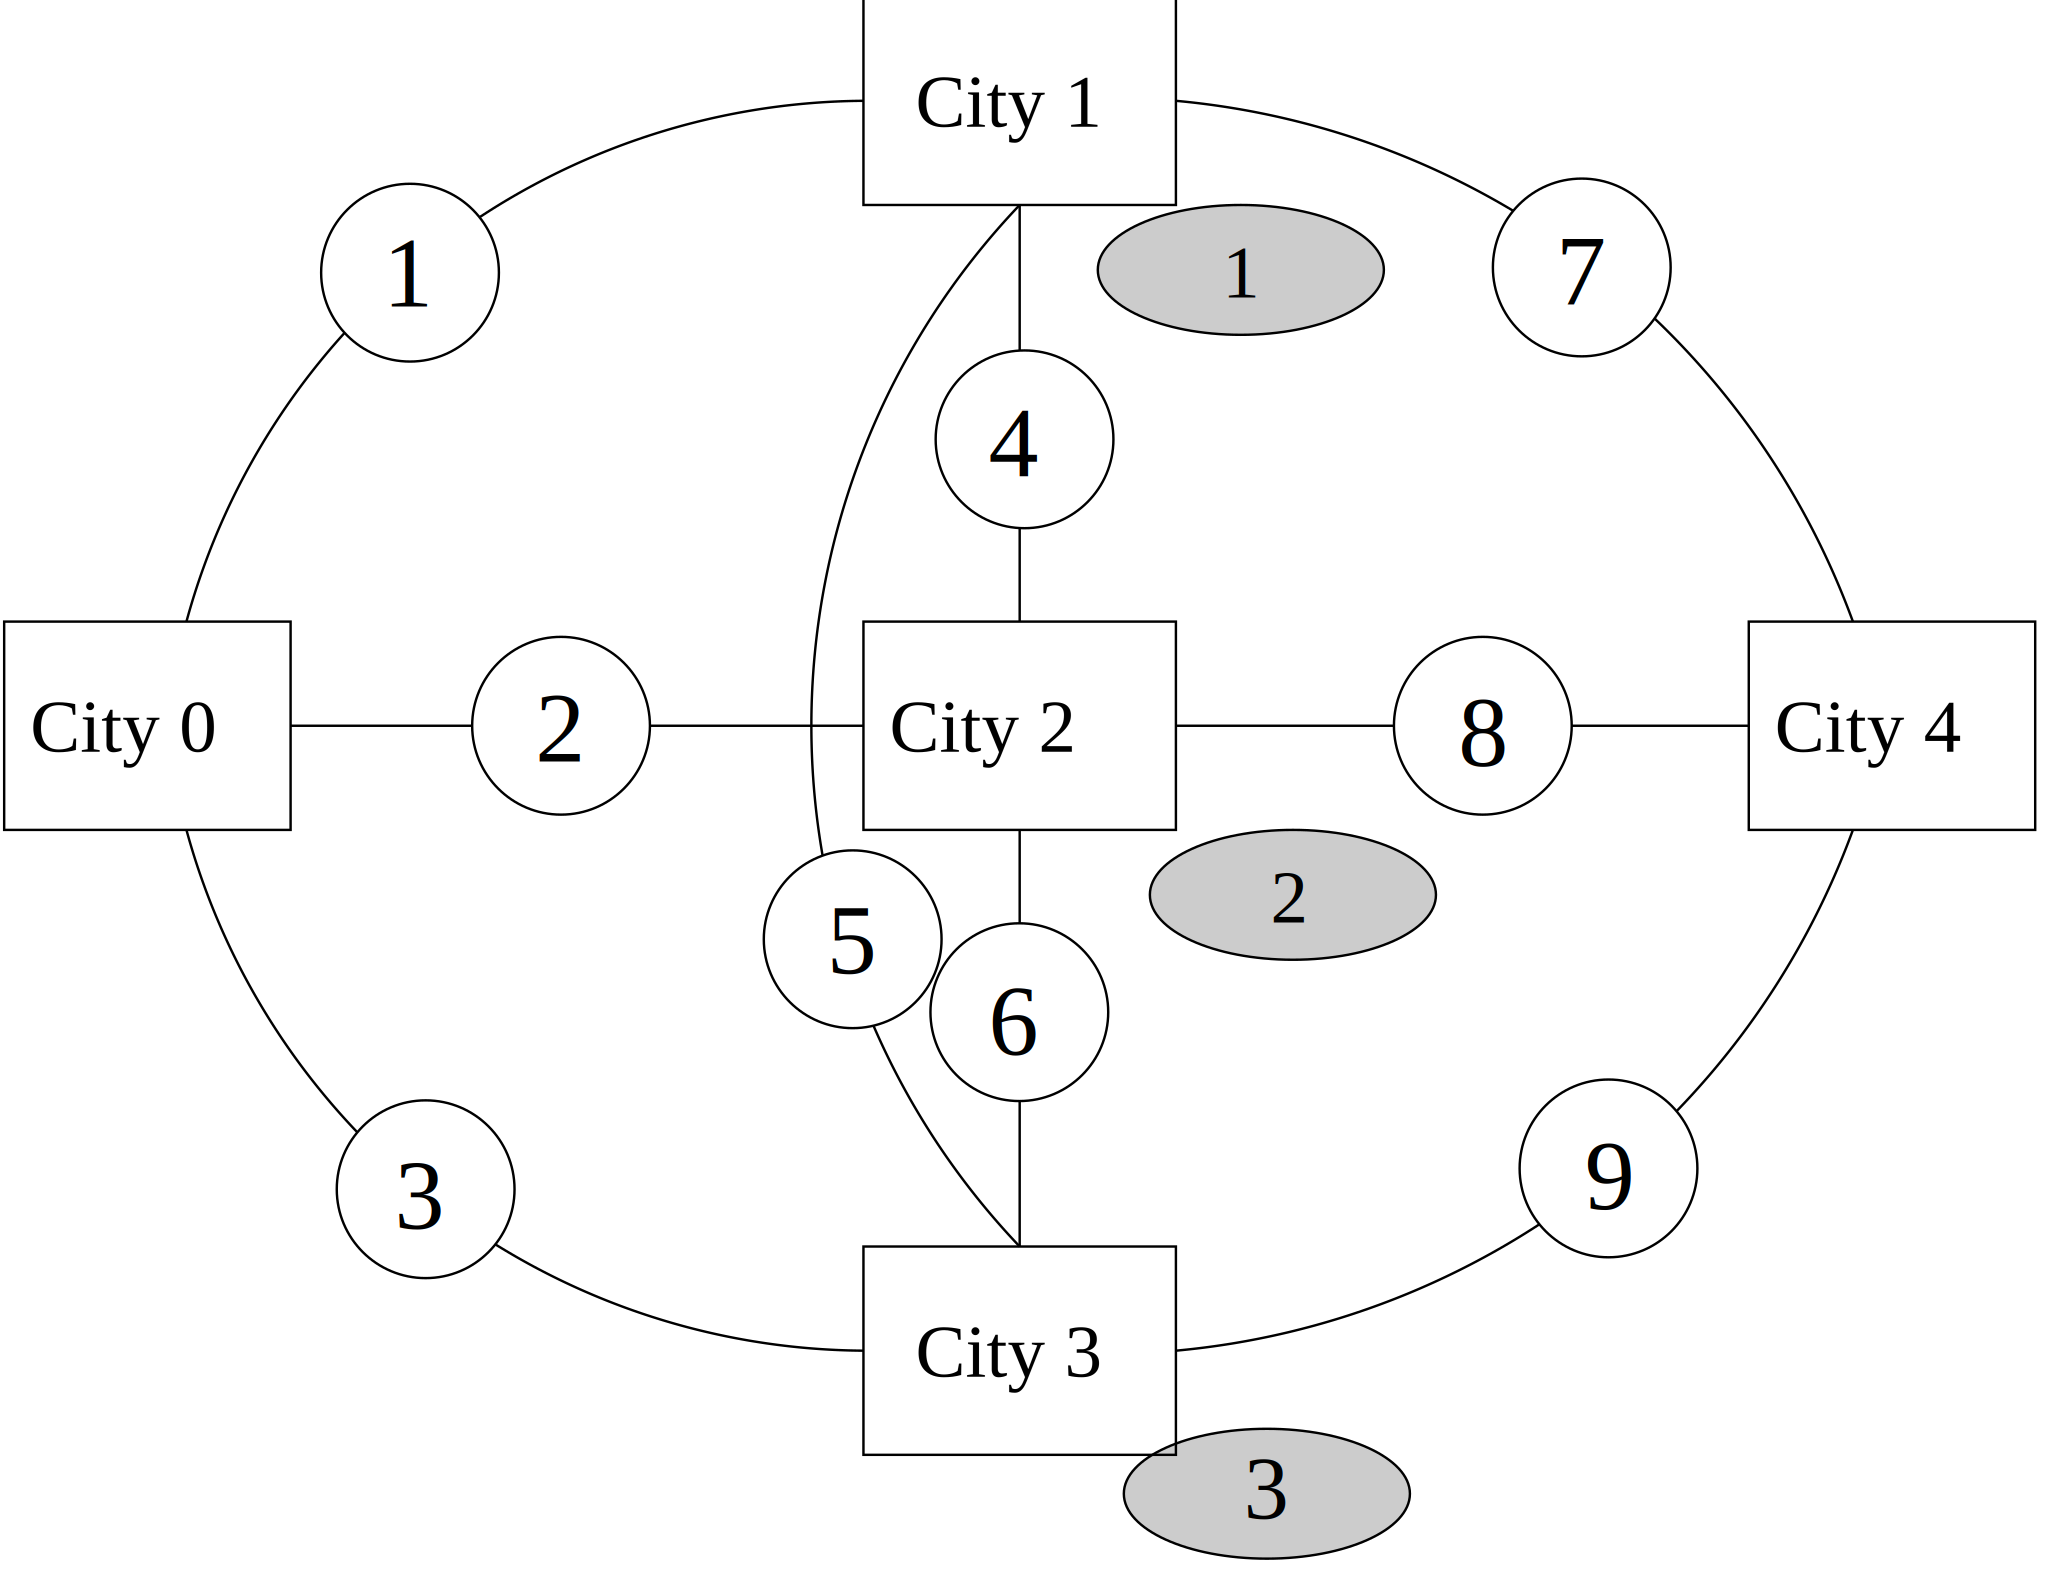
\includegraphics[width=0.5\columnwidth]{./generiqueMiniMulti.pdf}}
%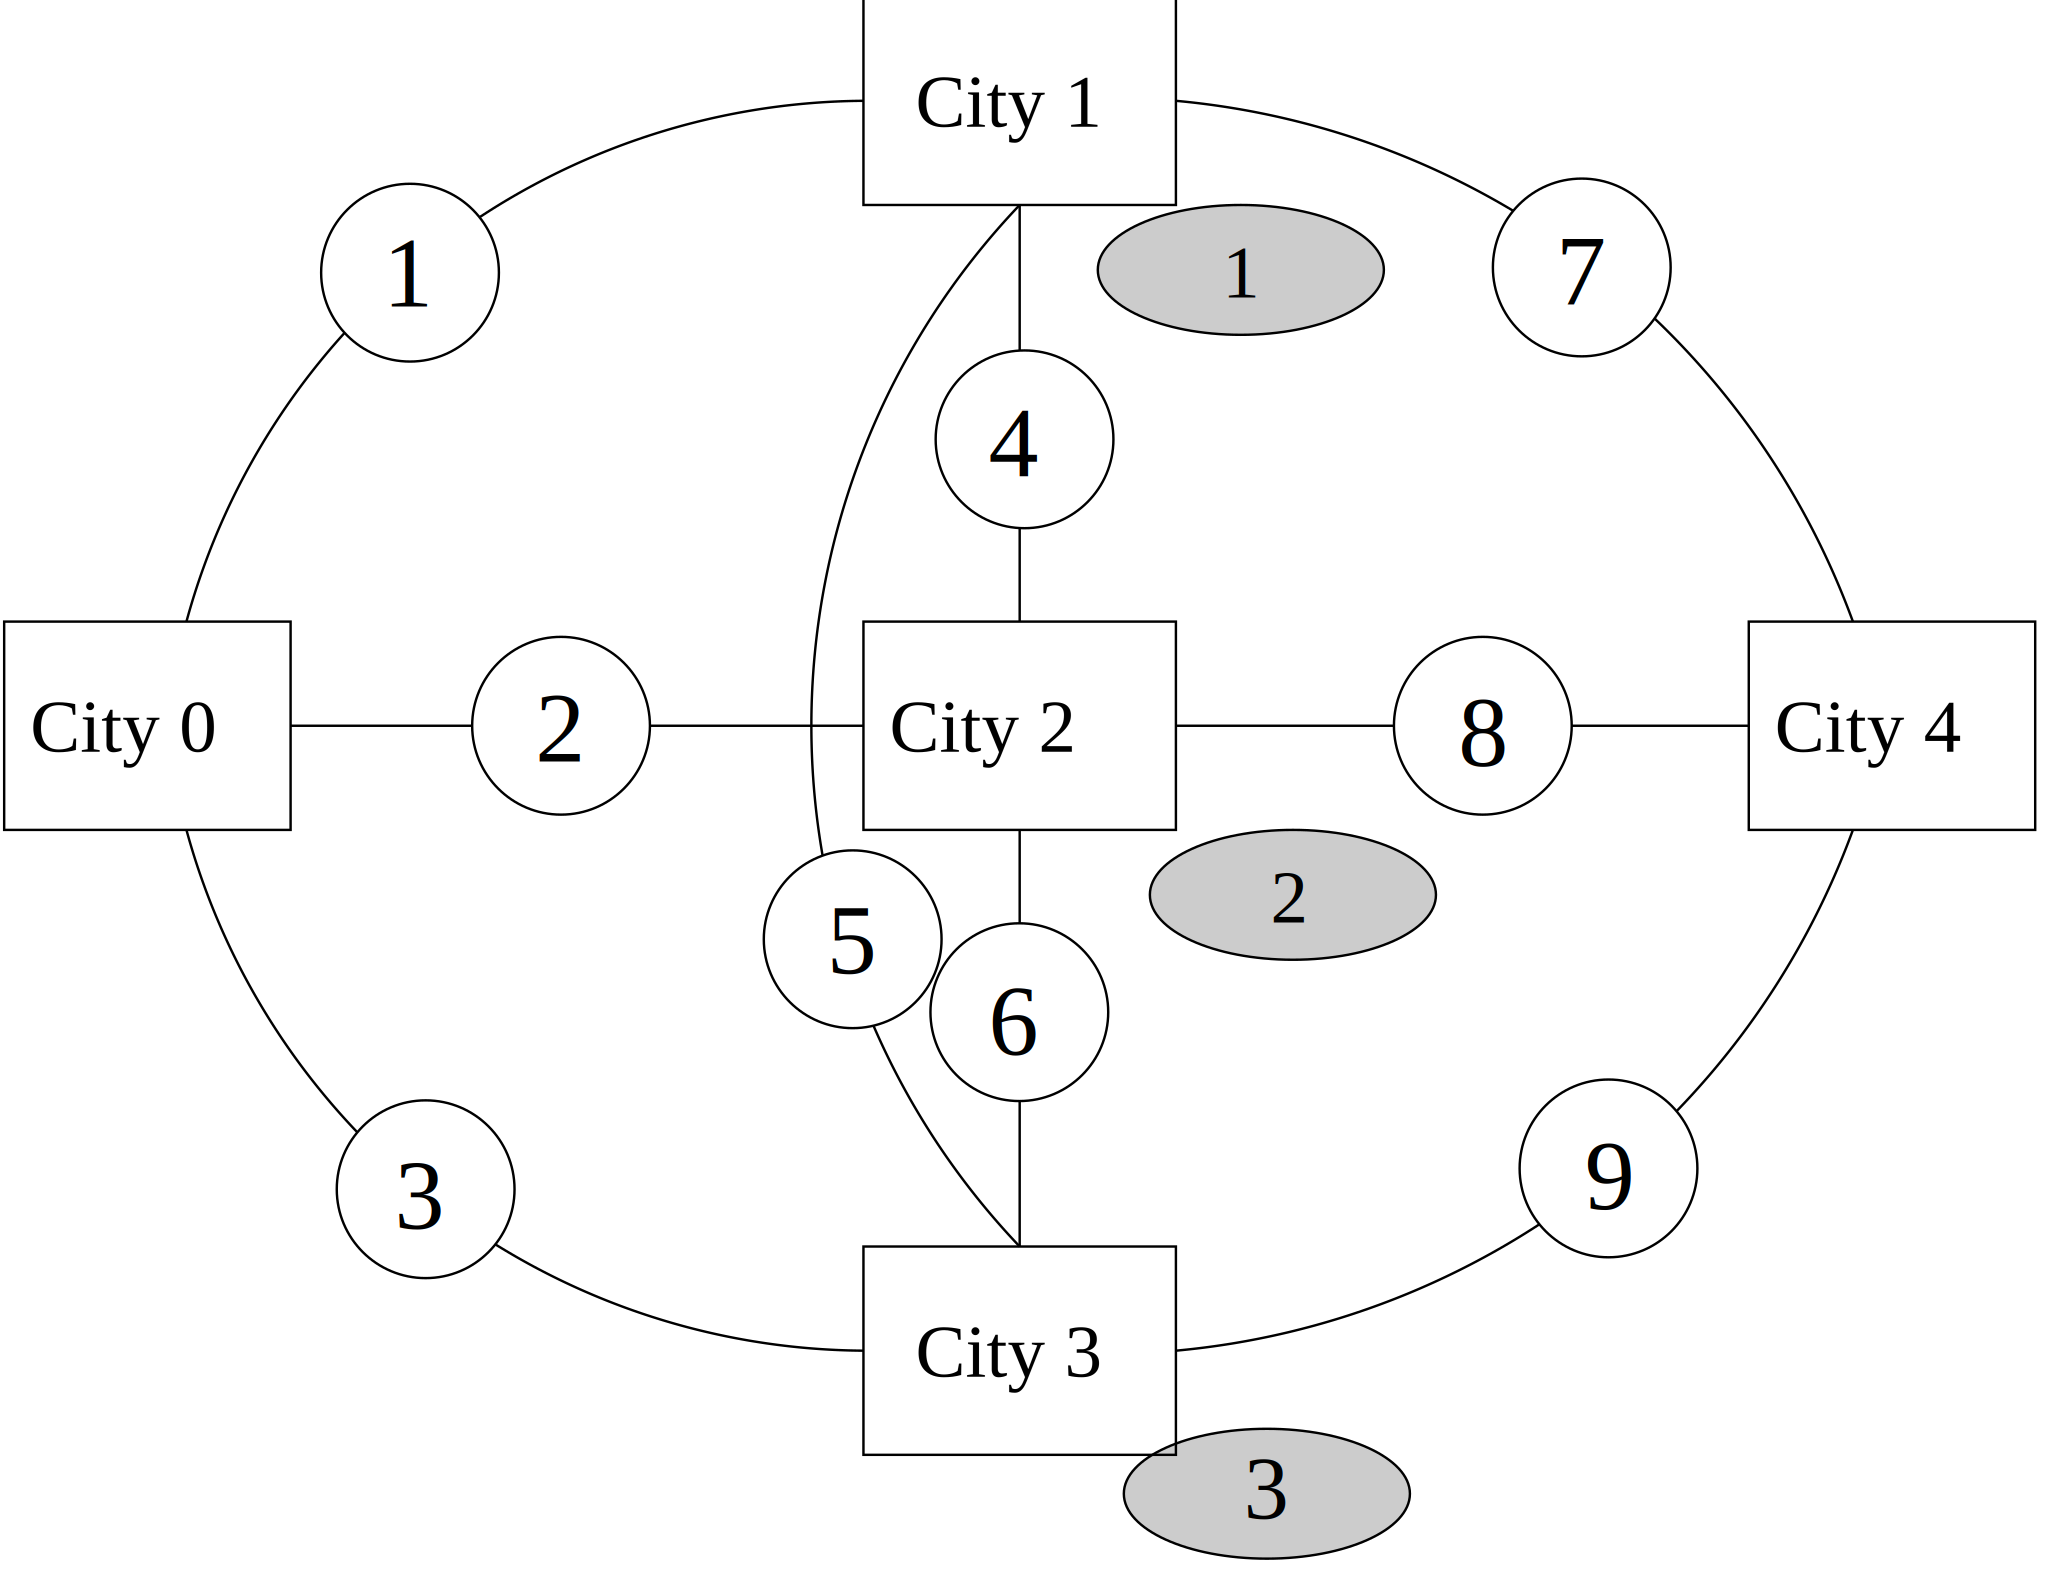
\includegraphics[height=0.5\columnwidth]{./generiqueMiniMulti.pdf} 
& 
\begin{tiny}
\begin{tabular}[t]{|m{.25cm}||m{.15cm}|m{.15cm}|m{.15cm}|}
\hline
Dur. & A & B & C \\
\hline 
1 & 2 & 2 & 2\\
2 & 4 & 4 & {\bf 3}\\
3 & 6 & 6 & {\bf 4}\\
4 & 3 & 3 & {\bf 1}\\
5 & 5 & 5 & {\bf 2}\\
6 & 3 & 3 & {\bf 1}\\
7 & 2 & 2 & 2\\
8 & 4 & 4 & {\bf 3}\\
9 & 6 & 6 & {\bf 4}\\
\hline \hline
Cost & & & \\
\hline
1 &  30 & 30 & 30\\
2 & 20 & {\bf 11} &{\bf 29}\\
3 & 10 & 10 & 10 \\
\hline
\end{tabular}
\end{tiny}
\end{tabular}
\caption{Schematic view, and 3 instances, of \MULTIZENO\ benchmark. Flight durations are attached to the possible routes (white circles), costs/risks are attached to landing in the central cities (grey circles). Three sets of values are given on the right, corresponding to Pareto fronts of Figure \ref{fig:allParetoFronts}. }
% \vskip -0.2cm
\label{fig:instance}
\end{figure}
\end{tiny}


\begin{figure}[tb]
\hskip -0.5cm
\begin{tabular}{cccc}
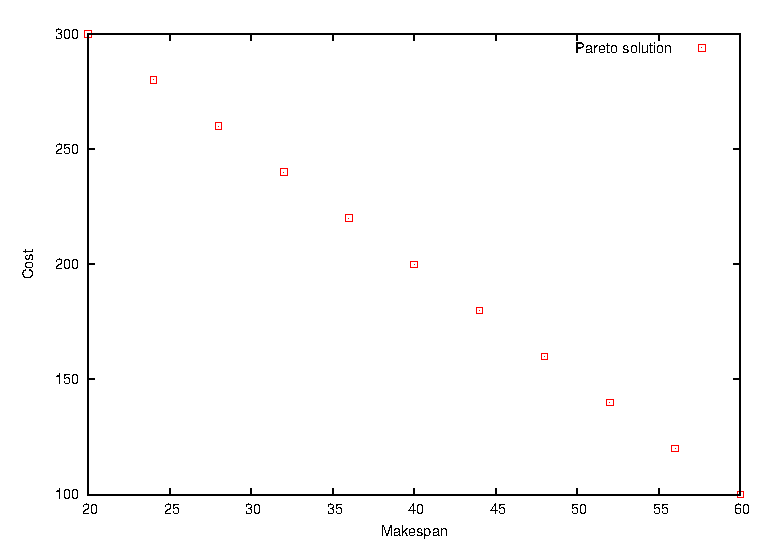
\includegraphics[width=0.32\columnwidth]{figures/zeno6e10} &
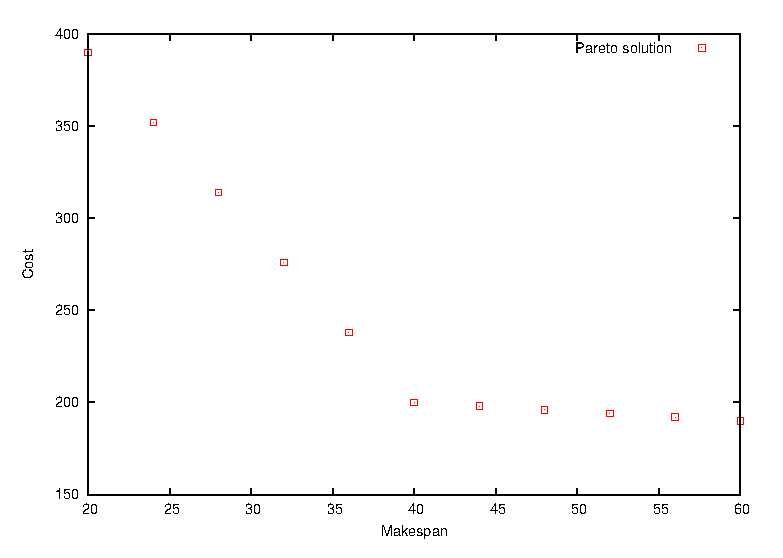
\includegraphics[width=0.32\columnwidth]{figures/zeno6di} &
% 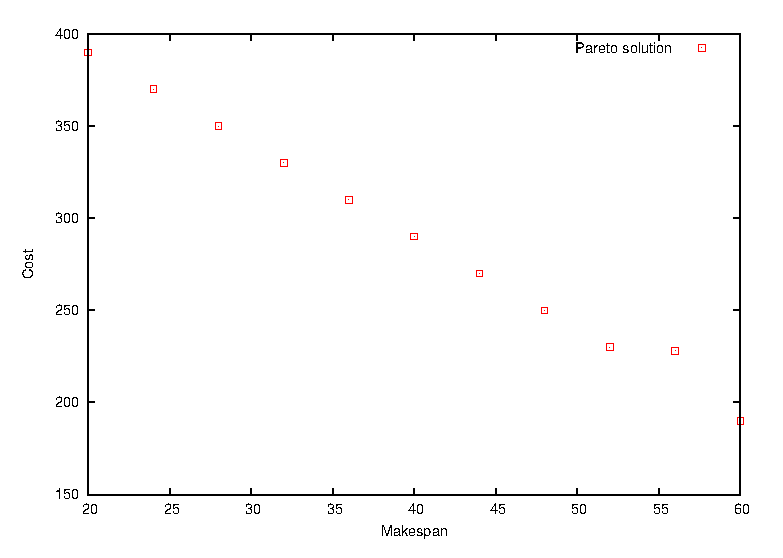
\includegraphics[width=0.24\textwidth]{../plot_archive/zeno6ds} &
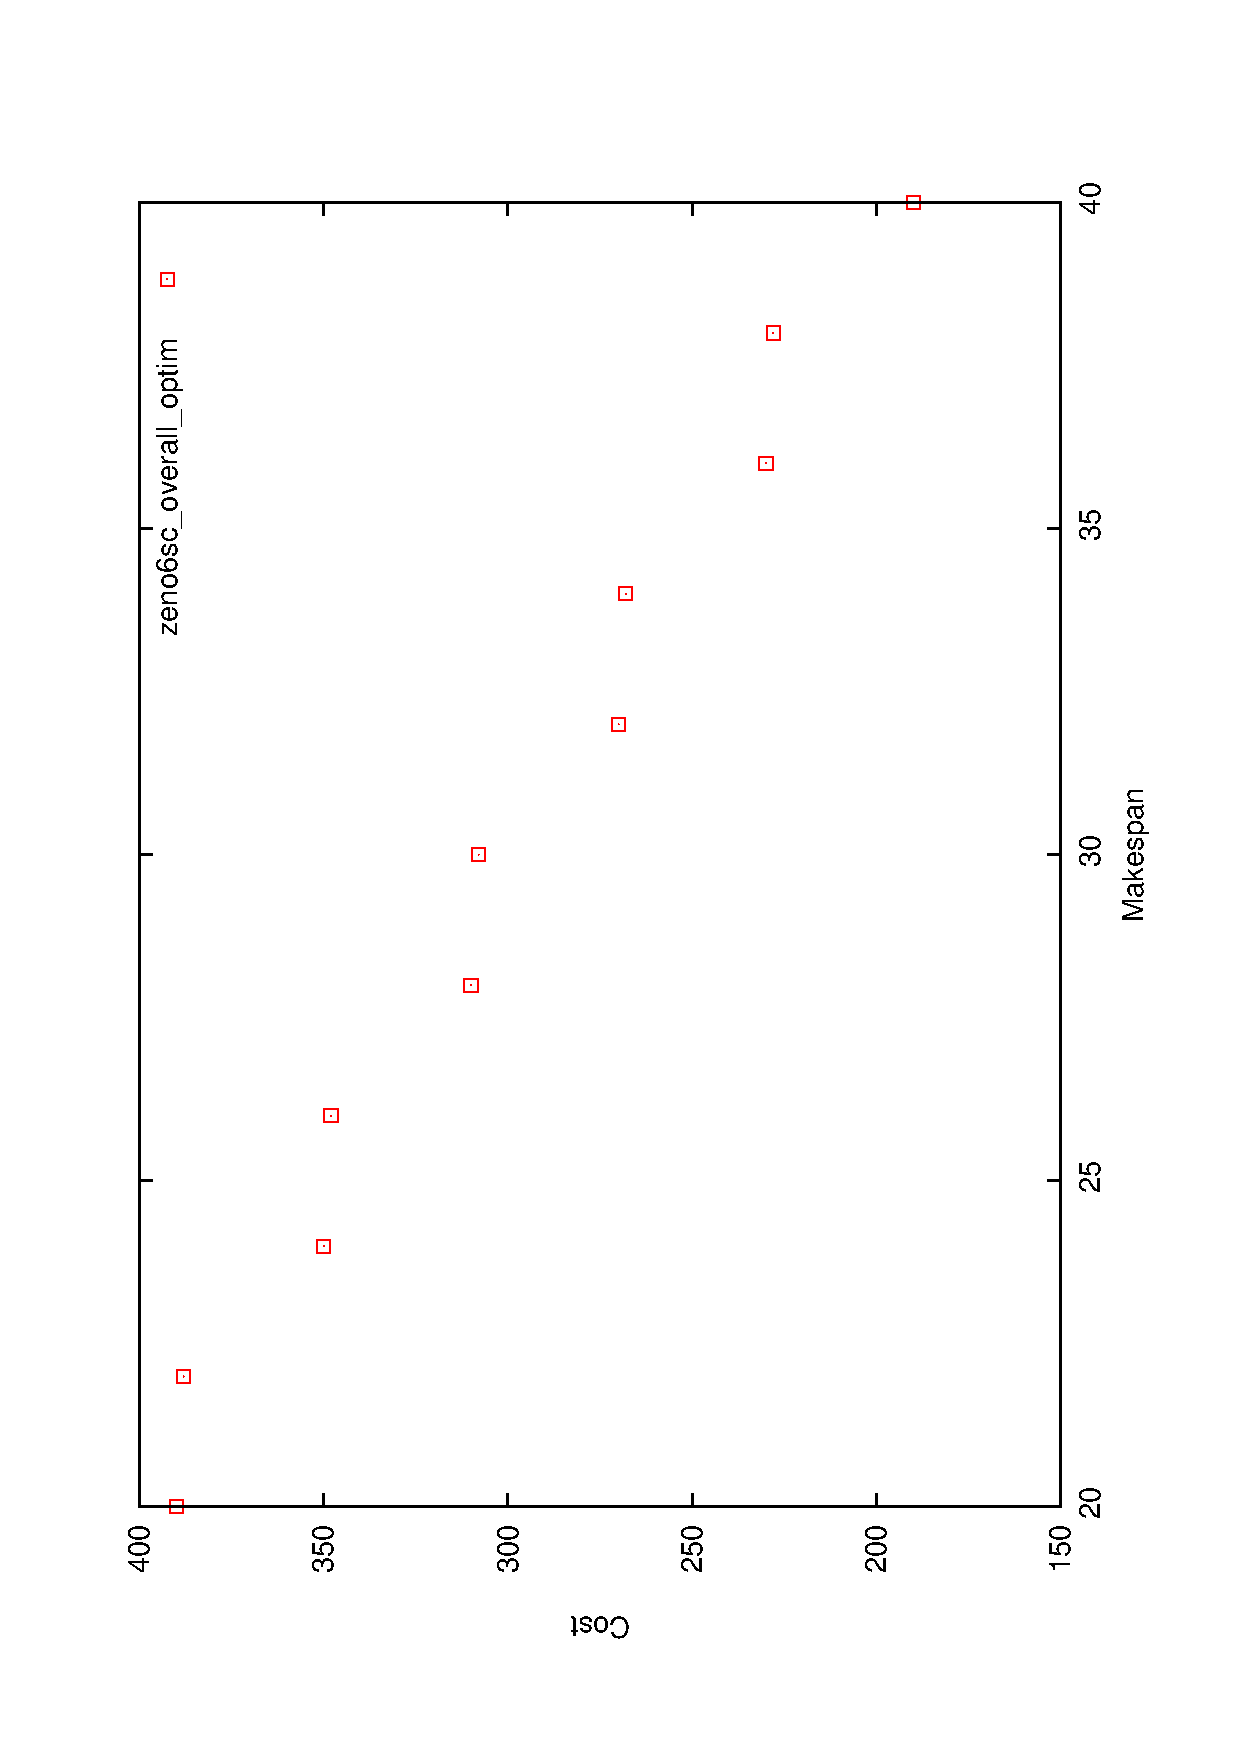
\includegraphics[width=0.32\columnwidth]{figures/zeno6sc}\\
A - Linear & B - Convex & C - Concave % & More concave 
\end{tabular}
\caption{Pareto fronts for the instances from Figure \ref{fig:instance}.}
\label{fig:allParetoFronts}
\end{figure}

The \MULTIZENO\ problem domain involves cities, passengers, and planes. One plane can carry at most one passenger from one city to another (action {\tt fly}), following an existing link of Figure \ref{fig:instance}, with corresponding flight durations (see Table). Costs are landing taxes for each of the middle cities. All instances in this work have 2 planes, all passengers are initially in {\tt city 0}, and must reach {\tt city 4}. The simplest non-trivial instance \MULTIZENO3 has 3 passengers. In its default configuration (column A in Table), the makespan-optimal solution has a total makespan of 8, as the reader will easily find out. But all flights have to land in {\tt city 1}, resulting in a cost of 120. The alternative route through  {\tt city 2} (resp. {\tt city 3}) has a makespan of 16 (resp. 24), and a cost of 80 (resp. 40). By increasing the number of passengers, and modifying the flight durations and landing costs, different trade-offs are made possible. Figure \ref{fig:allParetoFronts} displays 
the 3 exact Pareto fronts (in the makespan $\times$ cost space) corresponding to the durations and costs of the table in Figure \ref{fig:instance}, for a total of 6 passengers (aka \MULTIZENO6). 
Note that the second objective could also be considered as a {\em risk} \cite{nous-emo2013}, and the objective is then to minimize the maximum risk encountered during the execution of the plan. This variant of \MULTIZENO\ domain will not be considered here.

\subsection{Multi-Objectivization of IPC Problems}
\label{IPCbenchmarks}
Two satisficing tracks were open at IPC-2011: sequential satisficing, i.e., sequential STRIPS planning in which actions have a cost and where the total cost is to be minimized, and temporal satisficing, where actions have a duration and can be run in parallel and where the total makespan is to be minimized\footnote{\url{www.plg.inf.uc3m.es/ipc2011-deterministic}}.
Three possible ways of generating multiobjective instances have been considered. When the domains appeared in both tracks, with the same instances, and when the cost increases as the makespan decreases, a simple merge of both instances is enough. This was the case for domain \ELEVATORS.

% \begin{figure}
% \begin{tiny}
% \begin{verbatim}
% (:action move-up-slow
%    :parameters (?lift - slow-elevator ?f1 - count ?f2 - count)
%    :duration (= ?duration (travel-slow-temp ?f1 ?f2))
%    :precondition (and (lift-at ?lift ?f1) 
%                       (above ?f1 ?f2 )
%                       (reachable-floor ?lift ?f2) )
%    :effect (and (lift-at ?lift ?f2) 
%                 (not (lift-at ?lift ?f1)) 
%                 (increase (total-cost) (travel-slow-cost ?f1 ?f2))))
% \end{verbatim}
% \end{tiny}
% \caption{Typical action of multiobjective {\tt \ELEVATORS}.}
% \label{fig:elevator}
% \end{figure}


For some domains, the cost values of the cost instance did not ensure that both objectives would be antagonistic. This is the case for \CREWPLANNING, \FLOORTILE, and \PARCPRINTER. For these instances we arbitrarily set the cost values to a maximum cost minus the value of the duration. \FLOORTILE\ will be the typical domain from this category considered here.
Finally, for the \OPENSTACKS\ domain, the cost version has a single costly action, that penalizes the use of a new stack: such scheme is very general in scheduling applications with resources (with more resources, things get done faster, but cost more). For this domain, this cost action was simply added to the temporal domain.



\section{Experiments}
\label{sec:experiments}

The goal of the following experiments is to assess the efficiency of \MODAEYAHSP, and its robustness with respect to some variety of planning domains and the size of the instances. The instances presented in Section \ref{sec:benchmarks} will be used in turn, and the performance of \MODAEYAHSP\ will also be assessed against the baseline \MOLPG, the approach proposed in \citeauthor{LPG-PlanSIG2012} [\citeyear{LPG-PlanSIG2012}] (see Section \ref{sec:multi-planning}) which will also be evaluated. The experimental conditions will first be detailed.


\subsection{Parameter Tuning -- Experimental Conditions}
\label{sec:conditions}

\DAEYAHSP, and even more so, \MODAEYAHSP, have a number of free parameters that need to be tuned in order to obtain the best possible results. It is well-known that parameter tuning can make a complete difference between failure and success for the same algorithm on the same problem. In this work, all user-defined parameters have been tuned using the  framework \PARAMILS\
% \footnote{\url{http://www.cs.ubc.ca/labs/beta/Projects/ParamILS/}}~
\cite{ParamILS-JAIR}, that handles any parameterized algorithm whose parameters can be discretized, and uses some Iterated Local Search (ILS) to explore the space of parameter configurations.
Furthermore, because the goal of this work is to demonstrate the efficiency of \MODAE\ to robustly find a good approximation of the Pareto front of multiobjective AI Planning problems, those parameters were tuned anew for one instance of moderate complexity in each domain (see Section \ref{IPCbenchmarks}), and the resulting parameter set was used for all instances of the same domain. This represents a trade-off between CPU cost and performance: there is little hope to ever find some universal parameters for \DAE, that would allow \DAE\ to obtain its best quality performance on all possible instances; on the other hand, such best quality can obviously be obtained by optimizing the parameters anew for each new instance, but at the price of a huge CPU cost. On the other hand, following \citeauthor{LPG-PlanSIG2012} [\citeyear{LPG-PlanSIG2012}], within \MOLPG, LPG was ran in local-search mode, and given the same overall CPU time for its multiple restarts.


The main goal of the experiments presented here is to assess the ability of \MODAEYAHSP\ to find good quality approximations of the Pareto front. Hence the performance of the different algorithms will be reported w.r.t. the quality of the identified Pareto front after an arbitrary CPU time of 30 min (long enough to allow the algorithms to reach some steady population, as confirmed by preliminary runs). All runs were conducted on one core of the same 24-cores server with Xeon X5650@2.67GHz processors, running Ubuntu 10.04 Lucid.
\DAE\ was implement within the \PARADISEO\ framework \cite{paradiseo}. For all experiments, 11 independent runs were performed. All the performance assessment procedures, including the hypervolume calculations, have been achieved using the PISA performance assessment tool suite \cite{Bleuler2003}. % \footnote{\url{http://www.tik.ee.ethz.ch/pisa/}}. 


\subsection{Results on \MULTIZENO\ Instances}
\label{sec:resultsZENO}
Experiments have been conducted on the 3, 6 and 9 passengers versions of \MULTIZENO\ (Section \ref{ZenoBenchmarks}), with the Linear configuration (Figure \ref{fig:allParetoFronts}-a). The \MULTIZENO3 instance proved to be too easy, and both \MODAEYAHSP\ and \MOLPG\ could rapidly find the complete Pareto front. For \MULTIZENO6, the situation is drastically different for \MOLPG, that is only able to find a few points far away from the Pareto front (see Figure \ref{fig:zeno6-lpg-dae}). On the other hand, \MODAEYAHSP\ perfectly identifies the complete Pareto front in all runs for the ``Linear'' and ``Concave'' cases, while 2 runs out of 11 miss one point each in the ``Convex'' case. Finally, when tackling \MULTIZENO9 (and while \MOLPG\ fails to find a single feasible plan), \MODAEYAHSP\ is able to approach the true Pareto front rather robustly, as witnessed by Figure \ref{fig:zeno9-dae}, that represents the aggregated 11 Pareto fronts of the 11 independent runs.


\begin{figure*}[ht!]
   \subfloat[Importance of \YAHSP\ strategy]{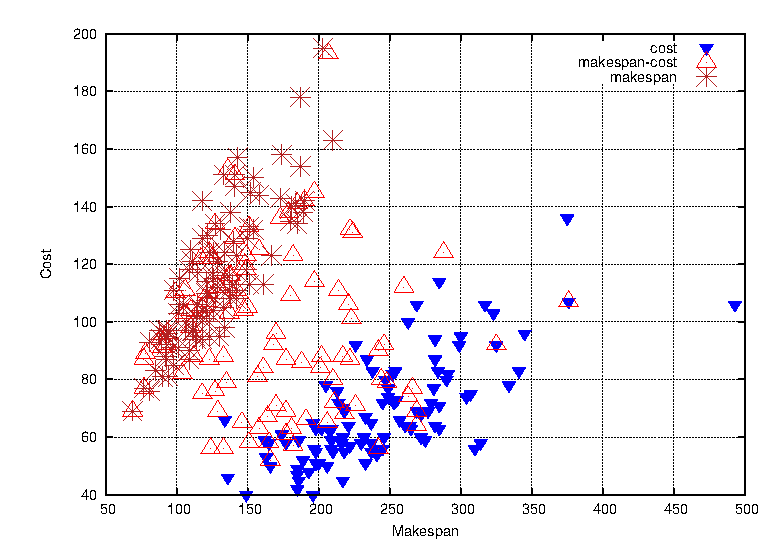
\includegraphics[width=0.32\textwidth,height=3.2cm\label{fig:strategies}] {figures/zeno9GlobLevelDaeYahsp_Add_dae_pareto1}}
 \subfloat[\MULTIZENO9: exact ($\bullet$) \& approx. ($\blacktriangledown$)\label{fig:zeno9-dae}]{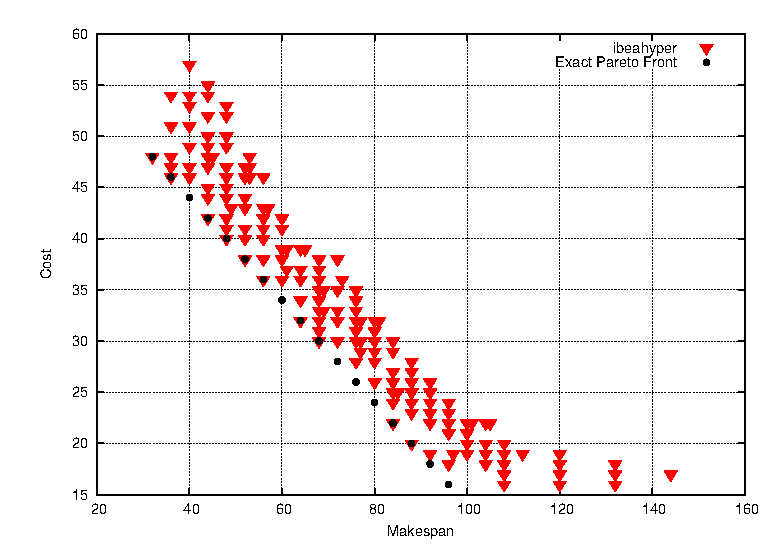
\includegraphics[width=0.32\textwidth,height=3.2cm]{figures/zeno9_Add_ibeahyper-pareto}}
 \subfloat[\MULTIZENO6: \DAE\ ($\blacktriangledown$) vs {\sc LPG} ($\vartriangle$)\label{fig:zeno6-lpg-dae}]{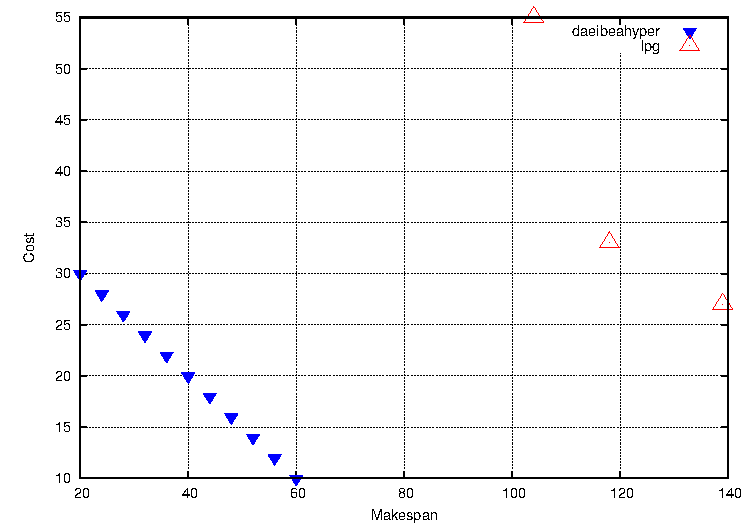
\includegraphics[width=0.32\textwidth,height=3.2cm]{figures/zeno6eMini_Add_dae_pareto}}
\caption{Experiments on \MULTIZENO\ instances (see text for details).}
\label{fig:paretoFronts}
\end{figure*}



\subsection{Results on Modified IPC-2011 Instances}
\label{sec:resultsIPC7}

\begin{figure*}[ht!]
  %\subfloat[openstacks05]{\label{openstacks05}\includegraphics[width=0.32\textwidth,height=3.2cm] {../plot_archive/p05_openstacks_Add_dae_pareto} }
  %\subfloat[openstacks10]{\label{openstacks10}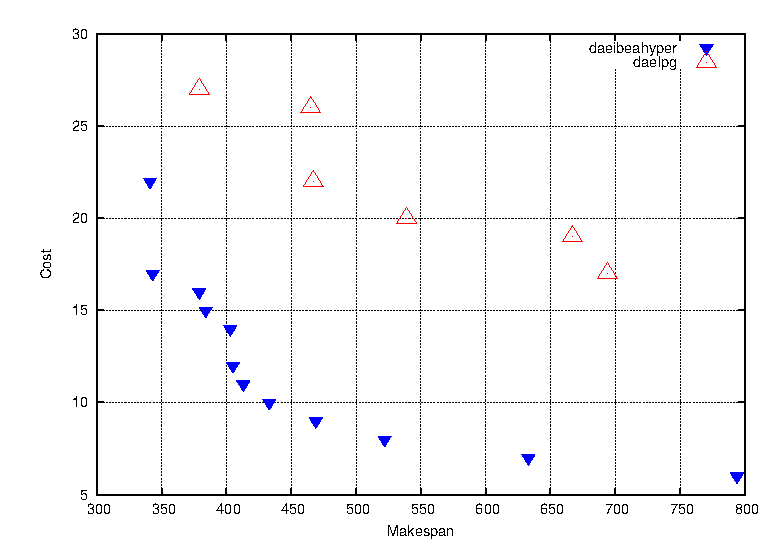
\includegraphics[width=0.32\textwidth,height=3.2cm]{../plot_archive/p10_openstacks_Add_dae_pareto}}
  \subfloat[\ELEVATORS01:\DAE\ ($\blacktriangledown$) vs {\sc LPG} ($\vartriangle$)]{\label{elevators01}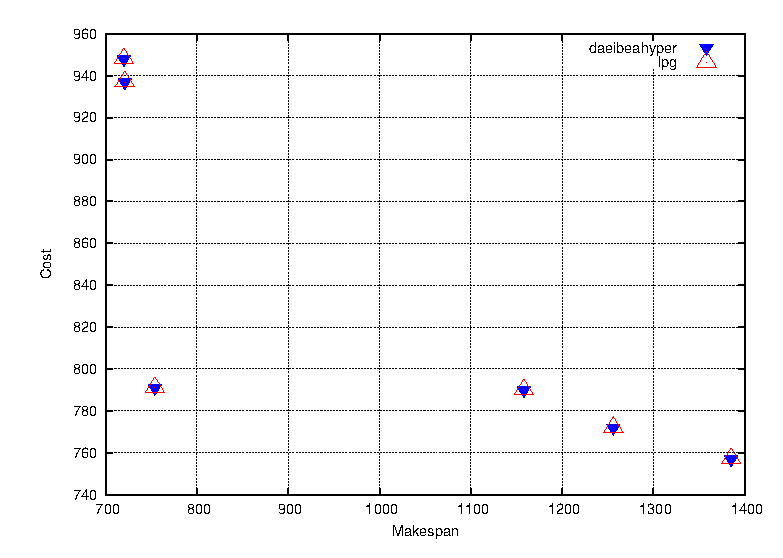
\includegraphics[width=0.32\textwidth,height=3.2cm] {figures/p01-p04_elevators_Add_dae_pareto} }
  \subfloat[\OPENSTACKS5: \DAE\ ($\blacktriangledown$) vs {\sc LPG} ($\vartriangle$)]{\label{openstacks5}\includegraphics[width=0.32\textwidth,height=3.2cm]{figures/p05_openstacks_Add_dae_pareto}}
  \subfloat[\FLOORTILE03: \DAE\ ($\blacktriangledown$) vs {\sc LPG} ($\vartriangle$)]{\label{floortile03}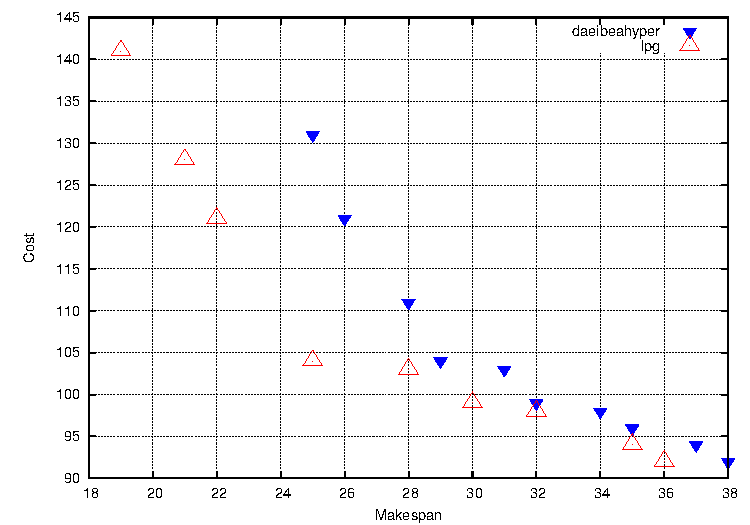
\includegraphics[width=0.32\textwidth,height=3.2cm] {figures/pfile3_floortile_Add_dae_pareto} }\\
  \subfloat[\ELEVATORS10: \DAE]{\label{elevators10dae}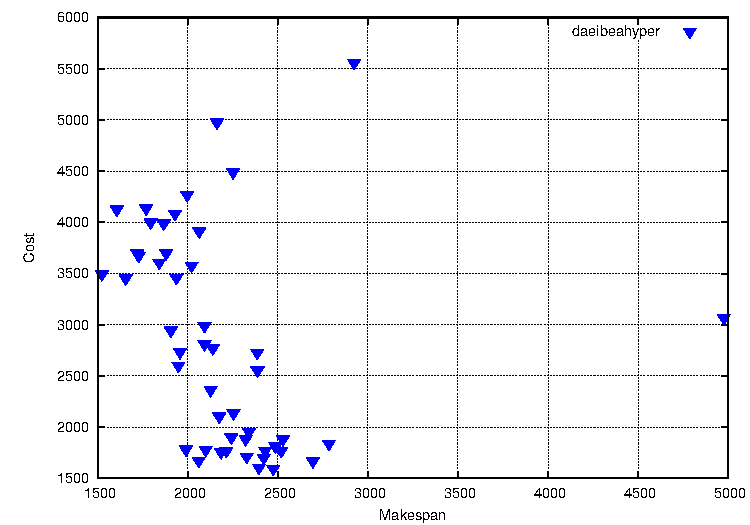
\includegraphics[width=0.32\textwidth,height=3.2cm]{figures/elevators_p10_Add_ibea_pareto} }
  \subfloat[\OPENSTACKS15: \DAE] {\label{openstacks15dae}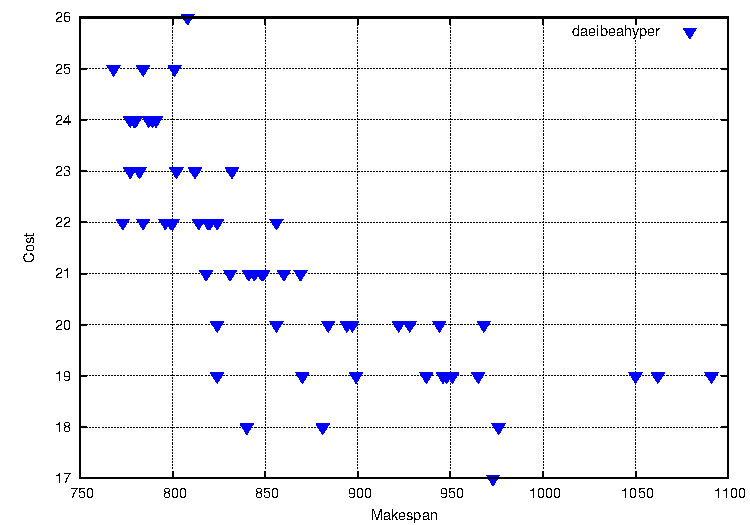
\includegraphics[width=0.32\textwidth,height=3.2cm]{figures/openstacks_p15_Add_ibea_pareto} }
  \subfloat[\OPENSTACKS15: LPG]{\label{openstacks15lpg}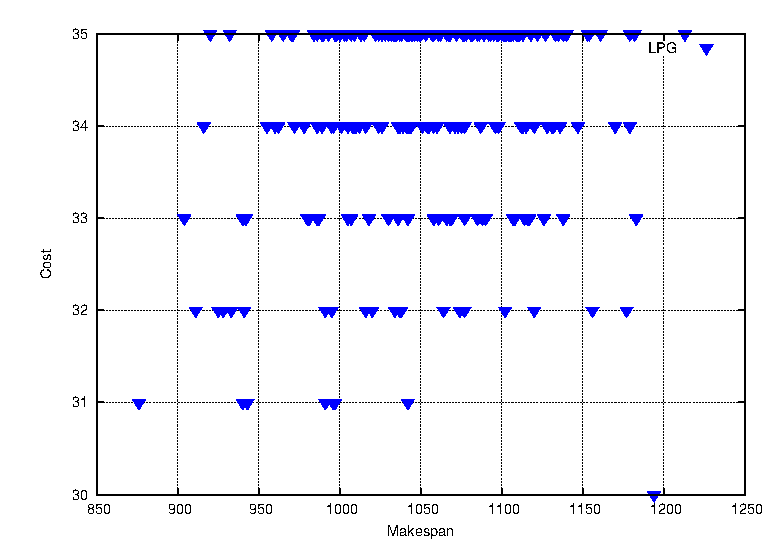
\includegraphics[width=0.32\textwidth,height=3.2cm]{figures/p15_openstacks_1000_lpg_pareto} }
\caption{Pareto fronts identified by \DAE\ and LPG for multi-objectivized IPC-2011 instances (a -- c) and complete solution sets found by \DAE\ (d and e) and by LPG (f), though displayed with different scales.}
\label{fig:ipc7}
\end{figure*}


Figure \ref{fig:ipc7} exhibits some results on multi-objectivized IPC-2011 instances (Section \ref{IPCbenchmarks}) for \MODAEYAHSP\ and \MOLPG. Indeed, because the exact Pareto front of these instances is unknown, the only possible assessment of \MODAEYAHSP\ is by comparison to \MOLPG\ results.

For the \ELEVATORS\ domain, instances 1, 5, 10 were experimented. For instance 1 (Figure \ref{elevators01}), \MODAEYAHSP\ and \MOLPG\ find exactly the same Pareto front, but \MOLPG\ is unable to find any solution for instances 5 and above. On the other hand, \MODAEYAHSP\ identifies some Pareto front, as can be seen for instance 10 on Figure \ref{elevators10dae}.

On the \OPENSTACKS\ domain, experiments involved instances 1, 5, 10, 15 and 20. For the small instances, 5 (Figure \ref{openstacks5}), and 1 and 10 (not shown), \MODAEYAHSP\ clearly finds a much better Pareto front than \MOLPG. For larger instances (15 and 20, not shown), the situation is even worse for \MOLPG, that only finds very poor solutions (w.r.t. the ones found by \MODAEYAHSP). As an illustration of how both algorithms explore the objective space, Figures \ref{openstacks15dae} and \ref{openstacks15lpg} show that the complete solution set computed by \DAE\ (merge of the 11 independent approximations) is nicely distributed along the Pareto front, whereas the solutions of LPG are much more scattered in the design space.

The situation changes for \FLOORTILE\ domain: instances 0, 3 and 4 were used, and here \MOLPG\ outperforms \MODAEYAHSP, as can be seen for instance 3 in Figure \ref{floortile03}.
However, as the instance size increases (instance 4 and above), the gap between LPG and \DAE\ decreases (not shown here).


\section{Discussion and Conclusion}
\label{sec:conclusion}

Not all planners are metric sensitive, in the sense advocated by \citeauthor{LPG-STAIRS2012} [\citeyear{LPG-STAIRS2012}]: the main contribution of this work is to demonstrate the ability of the \MODAE\ approach to turn any planner into a multiobjective planner, provided it can reason on either objectives alone (e.g., the makespan and the cost), as has been done here with \YAHSP. The resulting algorithm is a truly Pareto-based multiobjective planner, that consistently outperforms the \MOLPG\ metric-based approach on all instances tested here except the small \FLOORTILE\ instances. \MODAEYAHSP\ is able to solve much larger instances, and to find most of the time better approximations of the Pareto front than \MOLPG. 
More work is needed to improve even more the \MODAE\ approach to multiobjective planning. But we strongly believe that the rationale underlying the original \DAE\ is still valid, and that the decomposition-based approach that it implements will push upward the complexity of the problems that we can solve.

The second contribution of this work is the proposition for procedures to build multiobjective benchmark suites for AI Planning. There is no need to advocate the usefulness of large and diverse benchmark suites: in the context of single-objective optimization, advances in research (from the different versions of PDDL to the numerous powerful planners we know of today) have coevolved together with the design of the successive IPC benchmarks. Because multiobjective optimization is mandatory in order to tackle real-world problems, we strongly believe that progress in multiobjective planners requires as well the design of meaningful multiobjective AI Planning benchmarks with gradual difficulties. The \MULTIZENO\ suite detailed here is a first step in this direction: it is a tunable artificial testbed, and was shown to be able to generate interesting Pareto fronts (e.g. convex with a knee as well as non-convex). Furthermore, it has many degrees of freedom that still have not been explored: other combinations of 
durations and makespans, more intermediate cities, with more possible routes between them. 
Another possibility would have been to use the benchmarks designed by \citeauthor{LPG-PlanSIG2012} [\citeyear{LPG-STAIRS2012,LPG-PlanSIG2012}], but unfortunately the current implementation of \MODAEYAHSP\ relies on YAHSP, which does not handle numerical state variables except for the special case of action costs. However, we believe that multiobjective instances with time and cost objectives are already challenging enough, and could enable the use or extension of many more existing planners which mainly optimize cost or time.
The multi-objectivization of IPC-2011 domains is another possible route we have sketched, though more work is still required to transform the single-objective domains into ``interesting'' multiobjective ones, even in the favorable case where both a cost and a temporal version of the same domain already exist. When both objectives are not antagonistic enough, setting one as the inverse of the other does the trick, but the Pareto fronts remain close to linear fronts, while more interesting fronts (e.g. non-convex, ``discontinuous'', \ldots) are necessary to test different characteristics of the planners. 
Furthermore, such multiobjective instances can hardly be tackled by state-of-the-art metric sensitive planners, which are among the only potential competitors as of today: beside the general difficulty of finding the proper weights depending on the objective scales, linear combinations of the objectives can only give in that case one single non-dominated plan, and other aggregations are not guaranteed to lead to points on the Pareto front.
Final word on the modified IPC-2011 instances, the failure of LPG on even rather small instances suggests that we should probably have started with easiest instances (e.g., IPC-2008), since at IPC-2011 the easiest instances are significantly harder than those of IPC-2008.


\newpage
%% The file named.bst is a bibliography style file for BibTeX 0.99c
% \bibliographystyle{named}
% \bibliography{evobib}

\begin{thebibliography}{}

\bibitem[\protect\citeauthoryear{Biba{\"i} \bgroup \em et al.\egroup
  }{2010a}]{Bibai2010}
Jacques Biba{\"i}, Pierre Sav\'eant, Marc Schoenauer, and Vincent Vidal.
\newblock {An Evolutionary Metaheuristic Based on State Decomposition for
  Domain-Independent Satisficing Planning}.
\newblock In {R. Brafman et al.}, editor, {\em $20^{th}$ International
  Conference on Automated Planning and Scheduling (ICAPS-10)}, pages 18--25.
  AAAI Press, 2010.

\bibitem[\protect\citeauthoryear{Biba{\"i} \bgroup \em et al.\egroup
  }{2010b}]{bibai-EvoCOP2010}
Jacques Biba{\"i}, Pierre Sav\'eant, Marc Schoenauer, and Vincent Vidal.
\newblock {On the Benefit of Sub-Optimality within the Divide-and-Evolve
  Scheme}.
\newblock In Peter Cowling and Peter Merz, editors, {\em Proc. $10^{th}$
  EvoCOP}, pages 23--34. LNCS 6022, Springer Verlag, 2010.

\bibitem[\protect\citeauthoryear{Bleuler \bgroup \em et al.\egroup
  }{2003}]{Bleuler2003}
Stefan Bleuler, Marco Laumanns, Lothar Thiele, and Eckart Zitzler.
\newblock {PISA — A Platform and Programming Language Independent Interface
  for Search Algorithms}.
\newblock In {\em Evolutionary Multi-Criterion Optimization}, volume 2632 of
  {\em LNCS}, pages 494--508. Springer, 2003.

\bibitem[\protect\citeauthoryear{Deb}{2001}]{Deb-book}
K.~Deb.
\newblock {\em {Multi-Objective Optimization Using Evolutionary Algorithms}}.
\newblock John Wiley, 2001.

\bibitem[\protect\citeauthoryear{Do and Kambhampati}{2003}]{Do2003sapa}
M.B. Do and S.~Kambhampati.
\newblock {SAPA: A Multi-Objective Metric Temporal Planner}.
\newblock {\em J. Artif. Intell. Res. (JAIR)}, 20:155--194, 2003.

\bibitem[\protect\citeauthoryear{Eiben and Smith}{2003}]{EibenSmith2003}
A.E. Eiben and J.E. Smith.
\newblock {\em {Introduction to Evolutionary Computing}}.
\newblock Springer Verlag, 2003.

\bibitem[\protect\citeauthoryear{Fox and Long}{2003}]{PDDL2}
M.~Fox and D.~Long.
\newblock {PDDL2.1: An Extension to PDDL for Expressing Temporal Planning
  Domains}.
\newblock {\em J. Artif. Intell. Res. (JAIR)}, 20:61--124, 2003.

\bibitem[\protect\citeauthoryear{Gerevini and
  Long}{2006}]{gerevini2006preferences}
A.~Gerevini and D.~Long.
\newblock {Preferences and Soft Constraints in PDDL3}.
\newblock In {\em ICAPS Workshop on Planning with Preferences and Soft
  Constraints}, pages 46--53, 2006.

\bibitem[\protect\citeauthoryear{Gerevini \bgroup \em et al.\egroup
  }{2008}]{gerevini2008}
A.~Gerevini, A.~Saetti, and I.~Serina.
\newblock {An Approach to Efficient Planning with Numerical Fluents and
  Multi-Criteria Plan Quality}.
\newblock {\em Artificial Intelligence}, 172(8-9):899--944, 2008.

\bibitem[\protect\citeauthoryear{Haslum and
  Geffner}{2000}]{HaslumGeffner-AIPS-2000}
P.~Haslum and H.~Geffner.
\newblock Admissible {H}euristics for {O}ptimal {P}lanning.
\newblock In {\em $5^{th}$ Int. Conf. on AI Planning and Scheduling (AIPS
  2000)}, pages 140--149, 2000.

\bibitem[\protect\citeauthoryear{Hutter \bgroup \em et al.\egroup
  }{2009}]{ParamILS-JAIR}
Frank Hutter, Holger~H. Hoos, Kevin Leyton-Brown, and Thomas St\"{u}tzle.
\newblock {ParamILS: An Automatic Algorithm Configuration Framework}.
\newblock {\em J. Artif. Intell. Res. (JAIR)}, 36:267--306, 2009.

\bibitem[\protect\citeauthoryear{Khouadjia \bgroup \em et al.\egroup
  }{2013}]{nous-emo2013}
M.-R. Khouadjia, M.~Schoenauer, V.~Vidal, J.~Dr\'eo, and P.~Sav\'eant.
\newblock {Multi-Objective AI Planning: Evaluating DAE-YAHSP on a Tunable
  Benchmark}.
\newblock In {R. C. Purshouse et al.}, editor, {\em $7^{th}$ International
  Conference on Evolutionary Multi-Criterion Optimization (EMO 2013)}, LNCS.
  Springer Verlag, 2013.
\newblock To appear.

\bibitem[\protect\citeauthoryear{Liefooghe \bgroup \em et al.\egroup
  }{2007}]{paradiseo}
A.~Liefooghe, M.~Basseur, L.~Jourdan, and E.G. Talbi.
\newblock {ParadisEO-MOEO : A Framework for Evolutionary Multi-Objective
  Optimization}.
\newblock In {\em Evolutionary multi-criterion optimization}, pages 386--400.
  Springer, 2007.

\bibitem[\protect\citeauthoryear{Refanidis and Vlahavas}{2003}]{Refanidis03}
I.~Refanidis and I.~P. Vlahavas.
\newblock {Multiobjective Heuristic State-Space Planning}.
\newblock {\em Artificial Intelligence}, 145(1-2):1--32, 2003.

\bibitem[\protect\citeauthoryear{Schoenauer \bgroup \em et al.\egroup
  }{2006}]{evoCOP2006}
Marc Schoenauer, Pierre Sav{\'e}ant, and Vincent Vidal.
\newblock {Divide-and-Evolve: a New Memetic Scheme for Domain-Independent
  Temporal Planning}.
\newblock In J.~Gottlieb and G.~Raidl, editors, {\em Proc. $6^{th}$ EvoCOP},
  pages 247--260. LNCS 3906, Springer, 2006.

\bibitem[\protect\citeauthoryear{Sroka and Long}{2012a}]{LPG-STAIRS2012}
Michal Sroka and Derek Long.
\newblock {Exploring Metric Sensitivity of Planners for Generation of Pareto
  Frontiers}.
\newblock In K.~Kersting and M.~Toussaint, editors, {\em The Sixth "Starting
  Artificial Intelligence Research" Symposium (STAIRS 2012)}, pages 306--317.
  IOS Press, 2012.

\bibitem[\protect\citeauthoryear{Sroka and Long}{2012b}]{LPG-PlanSIG2012}
Michal Sroka and Derek Long.
\newblock {LPG Based System for Generation of Pareto Frontiers}.
\newblock In P.~Gregory, editor, {\em $30^{th}$ PlanSIG Workshop}, 2012.

\bibitem[\protect\citeauthoryear{Vidal and Geffner}{2004}]{vidal:aaai04}
V.~Vidal and H.~Geffner.
\newblock Branching and {P}runing: {A}n {O}ptimal {T}emporal {POCL} {P}lanner
  {B}ased on {C}onstraint {P}rogramming.
\newblock In {\em Nineteenth National Conference on Artificial Intelligence
  (AAAI-04)}, pages 570--577. AAAI Press, 2004.

\bibitem[\protect\citeauthoryear{Vidal}{2004}]{Vidal2004}
Vincent Vidal.
\newblock {A Lookahead Strategy for Heuristic Search Planning}.
\newblock In {\em $14^{th}$ International Conference on Planning and Scheduling
  (ICAPS-04)}, pages 150--159. AAAI Press, 2004.

\bibitem[\protect\citeauthoryear{Zitzler and K{\"u}nzli}{2004}]{Zitzler2004}
E.~Zitzler and S.~K{\"u}nzli.
\newblock {Indicator-Based Selection in Multiobjective Search}.
\newblock In {Xin Yao et al.}, editor, {\em $8^{th}$ International Conference
  on Parallel Problem Solving from Nature (PPSN VIII)}, pages 832--842. LNCS
  3242, Springer Verlag, 2004.

\end{thebibliography}
\end{document}

